\documentclass[11pt]{article}

\usepackage[margin=2.5cm]{geometry}
\usepackage{amsmath}
\usepackage{amssymb}
\usepackage{graphicx}
\usepackage{booktabs}
\usepackage{multirow}
\usepackage{hyperref}
\usepackage{xcolor}

\graphicspath{{../../plots/vector_search/}}

\newcommand{\Mpch}{\,h^{-1}\,\mathrm{Mpc}}
\newcommand{\FoM}{\mathrm{FoM}}
\newcommand{\code}[1]{\texttt{#1}}

\title{Technical note: searching the ASTRA quantile data vectors for the
largest Fisher gain over the full-sample 2PCF}
\author{ASTRA clustering project}
\date{June 2026}

\begin{document}
\maketitle

\begin{abstract}
Using the complete grid of full-box runs on disk (nine AbacusSummit
cosmologies $\times$ 50 HOD draws), we ask which ASTRA environment-split
statistic, or which pair of statistics, extracts the most cosmological
Fisher information beyond the plain full-sample auto-correlation.  We sweep
all 16 single quantile vectors and all 120 pairs, in two framings
(standalone and added to the full auto), scoring each by the
HOD-marginalised Fisher figure of merit.  The naive ranking is dominated by
the \emph{random}-quantile legs, with apparent gains up to $55\times$; we
show this is an artefact of unmodelled derivative noise in those
noise-limited legs (all of the global top~20 carry a random leg), not real
information.  Among the trustworthy \emph{data}-leg vectors the gains are
real but modest: adding a single full$\times$data-quantile cross buys
$\sim\!5\times$ in the three-parameter FoM, and the best clean pair
(\code{dQ1}$+$\code{xdQ1}, the void data auto and void data cross) reaches
$\sim\!14\times$, i.e.\ a factor $\sim\!2.4$ on each of
$\omega_b,\omega_c,n_s$.  We document the method, the artefact diagnosis,
and the honest ranking.
\end{abstract}

\section{Question and data}

ASTRA splits a galaxy sample into four environment quantiles
(Q1 underdense $\to$ Q4 overdense) and measures, per box, the
multipoles $\xi_{0,2}(s)$ of: the full-sample auto-correlation
(\code{tpcf\_full\_data}, our baseline), the four data-quantile autos
(\code{dQ1..4}), the four random-quantile autos (\code{rQ1..4}), the four
full$\times$data-quantile crosses (\code{xdQ1..4}), and the four
full$\times$random-quantile crosses (\code{xrQ1..4}).  That is
$17$ stems $\times\{\ell=0,2\}\times 15$ bins per run.

The signal data are the $9\times 50 = 450$ phase-matched full-box runs
(\code{data/fullbox/}); cosmology derivatives come from the global linear
response fit (\code{derivative\_global\_*}, condition number $1.34$ on the
full grid).  The covariance of one $500\Mpch$ subbox is estimated from the
mean-subtracted subboxes pooled across all nine cosmologies,
$9\times 64 = 576$ fluctuation samples, and scaled to the full
$2000\Mpch$ box volume ($C/64$).  The HOD nuisance covariance $C_{\rm HOD}$
is the empirical scatter of the 50 same-phase \code{c000} draws.

\section{Method}
\label{sec:method}

The analysis is implemented in \code{scripts/fisher\_vector\_search.py},
which reuses the assembly and Fisher machinery of
\code{scripts/fisher\_joint.py}.  The steps are:

\begin{enumerate}
\item \textbf{Candidate vectors.}  Each candidate is one or two ASTRA stems,
  taken at \emph{native} 15-bin resolution in mono$+$quad ($\ell=0,2$).  The
  576-sample pooled covariance keeps the Hartlap factor benign even at
  $n_b=60$ (pair) or $90$ (pair added to the full auto), so no rebinning is
  needed.  We evaluate the 16 singles and all $\binom{16}{2}=120$ pairs.
\item \textbf{Two framings.}  \emph{Standalone} scores the candidate by
  itself against the full auto (``is it better than the 2PCF?'').
  \emph{Additive} scores the full auto with the candidate appended
  (``what does ASTRA add to the 2PCF?'').  The additive framing is the
  physical measure of marginal information and is our headline.
\item \textbf{Fisher and marginalisation.}  For each candidate we build the
  $16\times16$ joint Fisher over the four cosmological parameters
  $\{\omega_b,\omega_c,n_s,\sigma_8\}$ and the twelve yuan23 HOD parameters,
  $F = D\,C^{-1}D^{\mathsf T}$ with Hartlap-corrected precision, add a
  Gaussian yuan23 prior on the HOD block, and read off the
  HOD-marginalised $4\times4$ cosmology covariance
  $\mathrm{Cov} = (F+F_{\rm prior})^{-1}_{[\rm cosmo]}$ (route a).
\item \textbf{Figure of merit.}  We reduce $\mathrm{Cov}$ to
  \begin{equation}
    \FoM_4 = \big[\det \mathrm{Cov}_{4}\big]^{-1/2}, \qquad
    \FoM_3 = \big[\det \mathrm{Cov}_{3}\big]^{-1/2},
  \end{equation}
  where $\mathrm{Cov}_3$ drops $\sigma_8$ (the upper-left $3\times3$ block,
  already marginalised over $\sigma_8$).  The \emph{gain} of a candidate is
  $\FoM/\FoM_{\rm full\,auto}$.  We headline $\FoM_3$ because the $\sigma_8$
  derivative is unreliable (Sec.~\ref{sec:caveat}), so a four-parameter FoM
  inherits that unreliability.
\end{enumerate}

\section{The random-leg trap}
\label{sec:caveat}

\begin{table}[t]
\centering
\caption{Raw top of the additive ranking (full auto $+$ stem(s)).  A star
marks a candidate that contains a random leg (\code{rQ} or \code{xrQ}).
\emph{Every} entry in the global top eight, and all 20 of the global top 20,
carry a random leg, despite random legs being the weakest tracers in every
earlier single-parameter test.}
\label{tab:raw}
\begin{tabular}{llrr}
\toprule
& vector & $\FoM_3$ gain & $\FoM_4$ gain \\
\midrule
\multirow{3}{*}{singles}
& \code{xrQ4}$^\star$        & 12.2 & 13.5 \\
& \code{rQ4}$^\star$         &  8.6 &  9.9 \\
& \code{xrQ1}$^\star$        &  7.8 &  8.6 \\
\midrule
\multirow{3}{*}{pairs}
& \code{xrQ1}$+$\code{xrQ4}$^\star$ & 55.8 & 64.6 \\
& \code{xdQ1}$+$\code{xrQ4}$^\star$ & 44.6 & 59.0 \\
& \code{xdQ4}$+$\code{xrQ4}$^\star$ & 43.4 & 60.3 \\
\bottomrule
\end{tabular}
\end{table}

Table~\ref{tab:raw} and the bright \code{rQ4}/\code{xrQ4}/\code{xrQ1} band
in Fig.~\ref{fig:heatmap} show that the naive sweep is dominated by random
legs, with implausible gains ($\FoM_3$ up to $55\times$, i.e.\ a factor
$\sim\!4$ on every parameter from one box).  This contradicts every prior
result, in which the underdense random leg was the \emph{weakest} vector and
carried the most derivative noise.  The resolution is that these gains are
an artefact:

\begin{itemize}
\item The random quantiles --- especially their quadrupoles --- are
  \emph{noise-limited}: their per-bin ASTRA-random scatter is comparable to
  the HOD-induced signal (measured separately: \code{rQ2/3} $\ell{=}2$ noise/
  signal $\approx 0.7$--$0.8$).  Their global-fit derivatives therefore
  contain large noise components.
\item A Fisher matrix treats the derivative $D$ as exact.  Noise in $D$ that
  is not represented in the data covariance $C$ inflates $D\,C^{-1}D^{\mathsf
  T}$: the Fisher reads derivative noise as constraining power, and a noisy
  derivative pointing in a direction nearly orthogonal to the full auto
  spuriously ``breaks'' degeneracies.
\item The signature is diagnostic: a random leg is barely better than the
  full auto on its own (\code{xrQ4} standalone $\FoM_3=1.6$) yet explodes
  when appended ($12\times$), and \emph{all} 20 top-20 vectors carry a
  random leg.  Real information would not concentrate so completely in the
  lowest-S/N legs.
\end{itemize}

We therefore flag every random-leg candidate and base the physical
conclusions on the data legs only.  Removing the random-leg artefact is
exactly the role of propagating the emulator derivative variance
(future work); it would deflate these spurious gains.

\section{The honest, data-leg ranking}
\label{sec:results}

\begin{table}[t]
\centering
\caption{Data-leg candidates only (no random leg).  Additive framing,
HOD-marginalised.  Baseline full-auto errors:
$\sigma(\omega_b)=5.7\times10^{-4}$,
$\sigma(\omega_c)=1.7\times10^{-3}$,
$\sigma(n_s)=1.3\times10^{-2}$,
$\sigma(\sigma_8)=1.4\times10^{-2}$.}
\label{tab:clean}
\begin{tabular}{llrrrr}
\toprule
& vector & $\FoM_3$ gain & $\sigma(\omega_b)$ & $\sigma(\omega_c)$ & $\sigma(n_s)$ \\
\midrule
\multirow{4}{*}{singles}
& \code{xdQ1} & 5.1 & $3.3\times10^{-4}$ & $8.4\times10^{-4}$ & $8.3\times10^{-3}$ \\
& \code{xdQ4} & 5.0 & $3.2\times10^{-4}$ & $8.4\times10^{-4}$ & $8.5\times10^{-3}$ \\
& \code{dQ4}  & 4.1 & $3.3\times10^{-4}$ & $9.8\times10^{-4}$ & $8.4\times10^{-3}$ \\
& \code{dQ1}  & 3.9 & $4.2\times10^{-4}$ & $1.1\times10^{-3}$ & $7.7\times10^{-3}$ \\
\midrule
\multirow{3}{*}{pairs}
& \code{dQ1}$+$\code{xdQ1} & 14.0 & $2.8\times10^{-4}$ & --- & $6.0\times10^{-3}$ \\
& \code{dQ2}$+$\code{xdQ1} & 12.8 & $2.5\times10^{-4}$ & --- & $4.9\times10^{-3}$ \\
& \code{xdQ3}$+$\code{xdQ4} & 12.2 & $2.6\times10^{-4}$ & --- & $5.0\times10^{-3}$ \\
\bottomrule
\end{tabular}
\end{table}

Restricting to data-leg candidates (Table~\ref{tab:clean},
Fig.~\ref{fig:singles}) gives a clean and physically sensible picture:

\begin{itemize}
\item \textbf{Singles.}  The full$\times$data-quantile crosses at the
  extremes lead --- \code{xdQ1} (void) and \code{xdQ4} (knot), $\FoM_3$ gain
  $\approx 5$ --- followed by the extreme data autos \code{dQ4}, \code{dQ1}
  ($\approx 4$).  The middle quantiles (Q2, Q3) are weaker.  Each of these
  improves $\omega_b$ and $n_s$ by $\sim\!1.6$--$1.7\times$ over the full
  auto.  Note that on its own each vector is \emph{worse} than the full auto
  (standalone $\FoM_3<1.1$); the gain is entirely degeneracy-breaking when
  added --- the ASTRA thesis.
\item \textbf{Pairs.}  The best clean pair is \code{dQ1}$+$\code{xdQ1} (void
  data auto $+$ void data cross), $\FoM_3$ gain $14$, i.e.\ a factor
  $\sim\!2.0$ on $\omega_b$ and $\sim\!2.2$ on $n_s$ over the full auto.
  Combinations of an extreme data auto with an extreme data cross dominate;
  pairs of two middle quantiles, or two stems from the same family, add
  little (redundant).
\item \textbf{$\sigma_8$ is untouched.}  No vector improves $\sigma_8$
  appreciably ($1.4\times10^{-2}\!\to\!\sim\!1.0\times10^{-2}$), consistent
  with $\sigma_8$ being amplitude-degenerate with the HOD and with its
  derivative being unreliable.  This is why $\FoM_3$ (which drops $\sigma_8$)
  is the trustworthy score; Fig.~\ref{fig:perparam} confirms the per-parameter
  picture.
\end{itemize}

\begin{figure}[t]
\centering
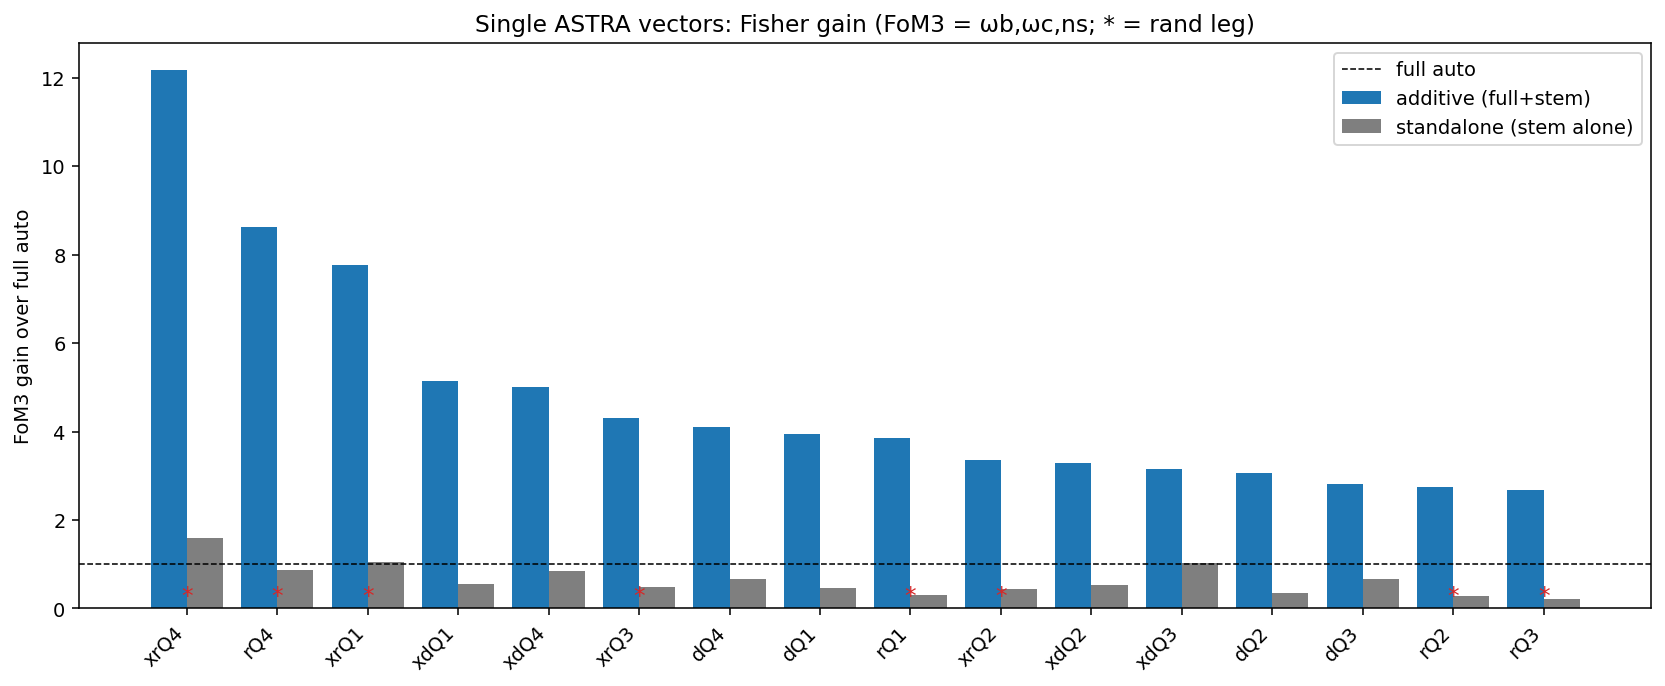
\includegraphics[width=0.92\textwidth]{single_vector_gains.png}
\caption{Single-vector $\FoM_3$ gain over the full auto, additive (blue) and
standalone (grey), ranked.  Red stars mark random-leg vectors, whose
additive gains are inflated by derivative noise (Sec.~\ref{sec:caveat}).
Every vector is at or below the full-auto line on its own; the gain is
degeneracy-breaking, realised only when appended.}
\label{fig:singles}
\end{figure}

\begin{figure}[t]
\centering
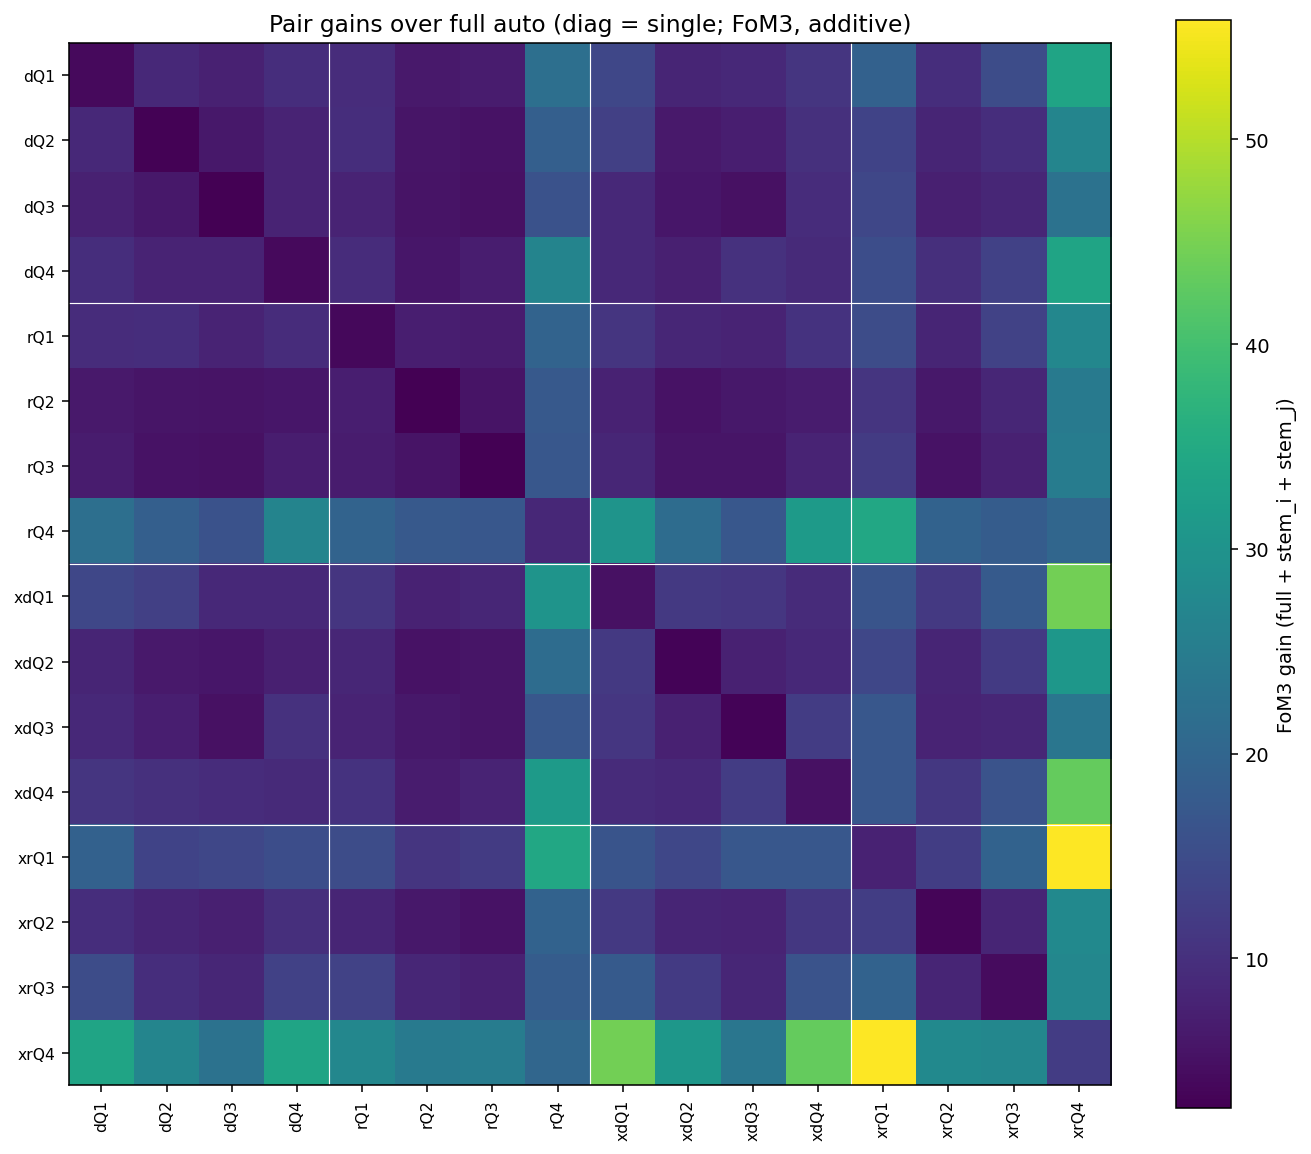
\includegraphics[width=0.78\textwidth]{pair_gain_heatmap.png}
\caption{Additive $\FoM_3$ gain for every pair, full auto $+$ stem$_i$ $+$
stem$_j$ (diagonal $=$ single).  White lines separate the four families
(\code{dQ}, \code{rQ}, \code{xdQ}, \code{xrQ}).  The bright band on the
\code{rQ4}/\code{xrQ4}/\code{xrQ1} rows and columns is the random-leg
artefact; the data-leg quadrants (\code{dQ}, \code{xdQ}) show the modest,
trustworthy gains.}
\label{fig:heatmap}
\end{figure}

\begin{figure}[t]
\centering
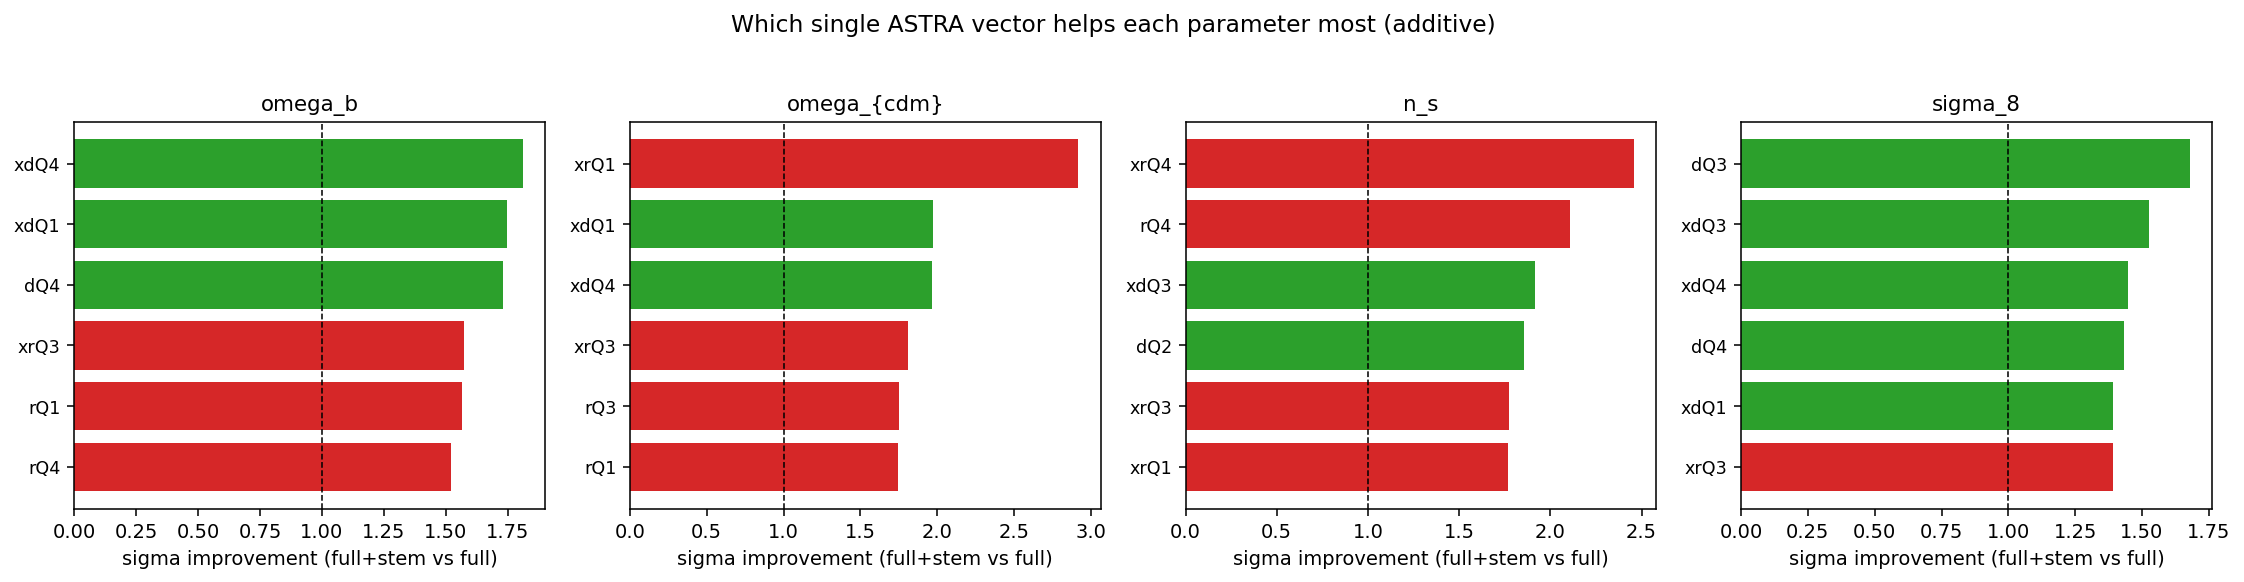
\includegraphics[width=\textwidth]{per_parameter_best.png}
\caption{For each cosmological parameter, the single ASTRA vectors that most
improve its marginalised error when added to the full auto.  Green bars are
data-leg vectors (trustworthy); red bars are random-leg vectors (artefact).}
\label{fig:perparam}
\end{figure}

\section{Conclusions}

\begin{enumerate}
\item The systematic sweep of all 16 singles and 120 pairs is dominated, at
  face value, by random-leg vectors with gains up to $55\times$.  This is a
  \textbf{derivative-noise artefact}, not physics: the noise-limited random
  legs have noisy global-fit derivatives that the Fisher misreads as
  information.  Any data-vector ranking on this grid must exclude or
  noise-correct the random legs.
\item Among the \textbf{trustworthy data legs}, the full$\times$data-quantile
  crosses at the density extremes (\code{xdQ1}, \code{xdQ4}) are the best
  single additions ($\FoM_3$ gain $\approx 5$), and the best clean pair is
  the void data auto with the void data cross, \code{dQ1}$+$\code{xdQ1}
  ($\FoM_3$ gain $14$, $\sim\!2.4\times$ per parameter on
  $\omega_b,\omega_c,n_s$).  The gains are pure degeneracy breaking: each
  vector is worse than the full auto alone.
\item $\sigma_8$ is not improved by any vector, consistent with its
  HOD-amplitude degeneracy and unreliable derivative.
\item \textbf{Next steps.}  (i) Propagate the GP emulator derivative variance
  (calibrated with the $\sim\!1.25\times$ inflation measured separately) so
  the random-leg artefact is deflated and the random legs can be ranked
  honestly; (ii) use the higher-iteration runs to denoise the random-quantile
  derivatives directly; (iii) revisit the four-parameter FoM once a
  trustworthy $\sigma_8$ derivative is available.
\end{enumerate}

All numbers are reproduced by
\code{python scripts/fisher\_vector\_search.py}; the full ranked table is in
\code{plots/vector\_search/vector\_search\_results.csv}.

\end{document}
